\section{Conformance Checking}
\subsection{Replay-based Conformance Checking}
\begin{exercise}{1}
Given the following Petri net and event log:
\begin{figure}[H]
    \centering
    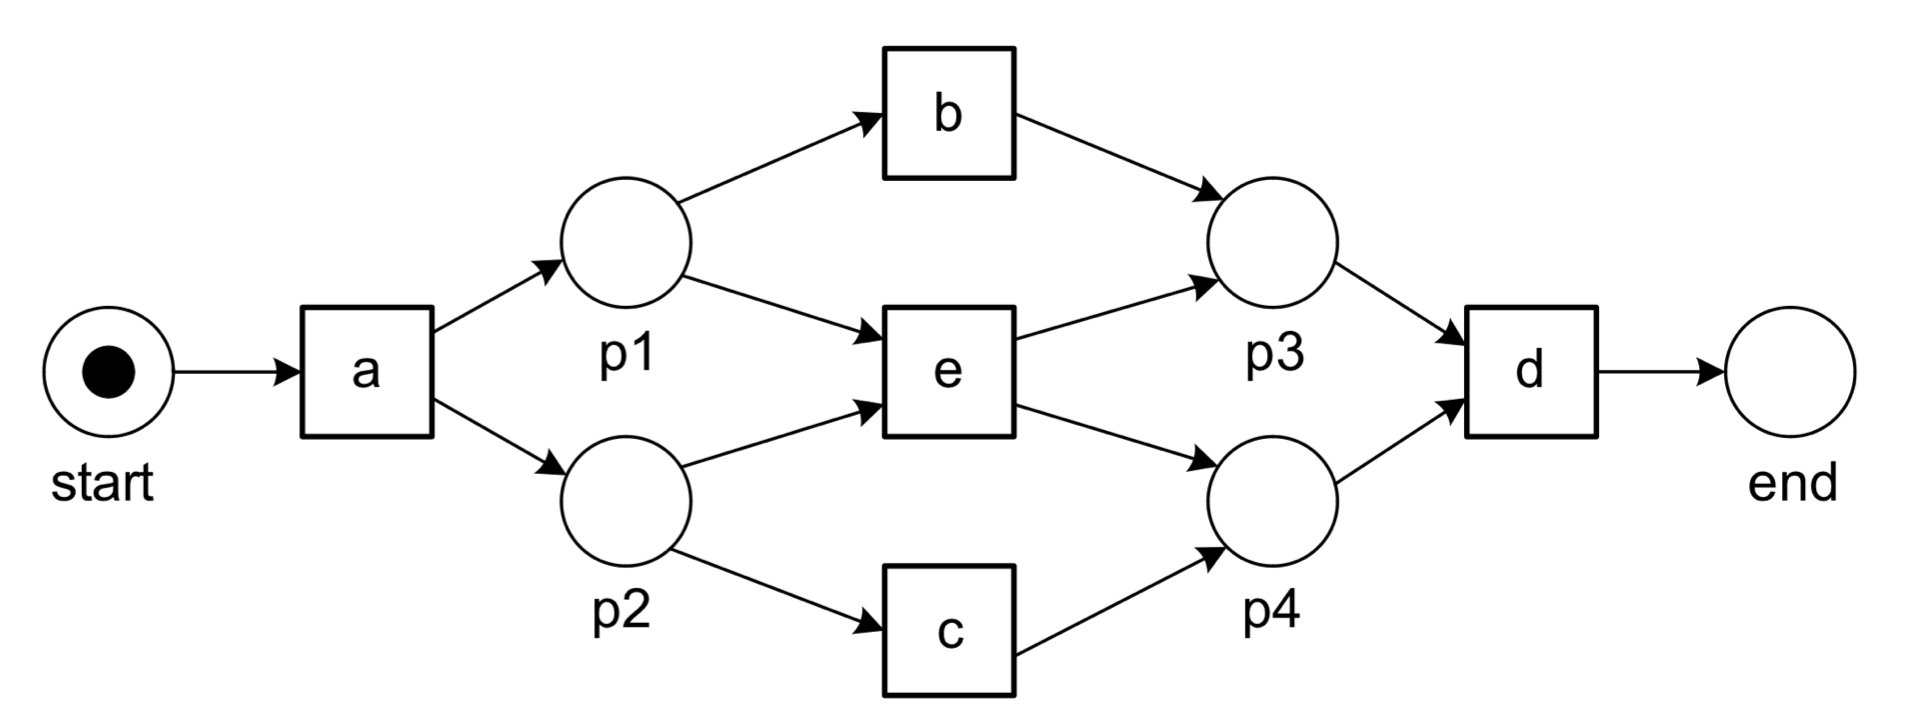
\includegraphics[width=0.4\textwidth]{../images/exercises/replay_based-1.png}
    \caption{Petri net for Exercise 1}
\end{figure}
\[L = [\langle a,b,c,d \rangle^{10}, \langle a,c,b,d \rangle^{10}, \langle a,e,d \rangle^{10}, \langle a,b,d \rangle^{2}, \langle a,c,d \rangle^{1},\]
\[ \langle a,d \rangle^{1}, \langle a,b,b,d \rangle^{1}\]
Use replay-based conformance checking to compute the fitness of the event log with respect to the Petri net.
\end{exercise}
\paragraph{Solution:}
\begin{enumerate}
    \item First, we replay each unique trace in the event log on the Petri net and collect the statistics:
    \begin{itemize}
        \item For trace $\langle a,b,c,d \rangle$:
        \begin{itemize}
            \item We first produce a token in place $start$ ($p=1$);
            \item We then fire transition $a$, consuming the token from place $start$ and producing a token in each of the output places of $a$ ($c=1$, $p=3$);
            \item We then fire transition $b$, consuming a token from place $p_1$ and producing a token in $p_3$ ($c=2$, $p=4$);
            \item We then fire transition $c$, consuming a token from place $p_2$ and producing a token in $p_4$ ($c=3$, $p=5$);
            \item We then fire transition $d$, consuming tokens from places $p_3$ and $p_4$ and producing a token in place $end$ ($c=5$, $p=6$);
            \item Finally, we consume the token from place $end$ ($c=6$, $p=6$);
        \end{itemize}
        \item For trace $\langle a,c,b,d \rangle$, we have the same statistics as above: $p=6$, $c=6$, $m=0$, $r=0$;
        \item For trace $\langle a,e,d \rangle$, we have $p=6$, $c=6$, $m=0$, $r=0$;
        \item For trace $\langle a,b,d \rangle$, we have $p=5$, $c=5$, $m=1$, $r=1$;
        \item For trace $\langle a,c,d \rangle$, we have the same statistics as above: $p=5$, $c=5$, $m=1$, $r=1$;
        \item For trace $\langle a,d \rangle$, we have $p=4$, $c=4$, $m=2$, $r=2$;
        \item For trace $\langle a,b,b,d \rangle$, we have $p=6, c=6, m=2, r=2$;
    \end{itemize}
    \item Now, we can sum the statistics weighted by the frequency of each trace in the event log:
    \begin{itemize}
        \item $P_{total} = 10 \times 6 + 10 \times 6 + 10\times 6 + 2\times 5 + 1\times 5 + 1\times 4 + 1\times 6 = 205$;
        \item $C_{total} = 205$ since every trace has the same number of produced and consumed tokens;
        \item $M_{total} = 0 + 0 + 0 + 1 \times 2 + 1 + 2 + 2 = 7$;
        \item $R_{total} = 7$ since the remaining tokens are equal to the missing tokens for each trace.
    \end{itemize}
    \item Finally, we can compute the fitness of the event log using the formula:
    \[Fitness_{Log} = \frac{1}{2} (1 - \frac{M_{total}}{C_{total}}) + \frac{1}{2} (1 - \frac{R_{total}}{P_{total}}) = \frac{1}{2} (1 - \frac{7}{205}) + \frac{1}{2} (1 - \frac{7}{205}) = \]
    \[ = 1 - \frac{7}{205} = \frac{198}{205} \approx 0.9659\]
\end{enumerate}

\begin{exercise}{2}
Given the following event log:
\[L = [\langle a,b,d,e,f \rangle^{10}, \langle a,c,e,d,f \rangle^{10} ]\]
\begin{enumerate}
    \item Construct the Petri net using the Alpha Miner algorithm;
    \item Use replay-based conformance checking to compute the fitness of the event log with respect to the Petri net.
\end{enumerate}
\end{exercise}
\paragraph{Solution:}

\begin{exercise}{3}
Given the following Petri net and event log:
\begin{figure}[H]
    \centering
    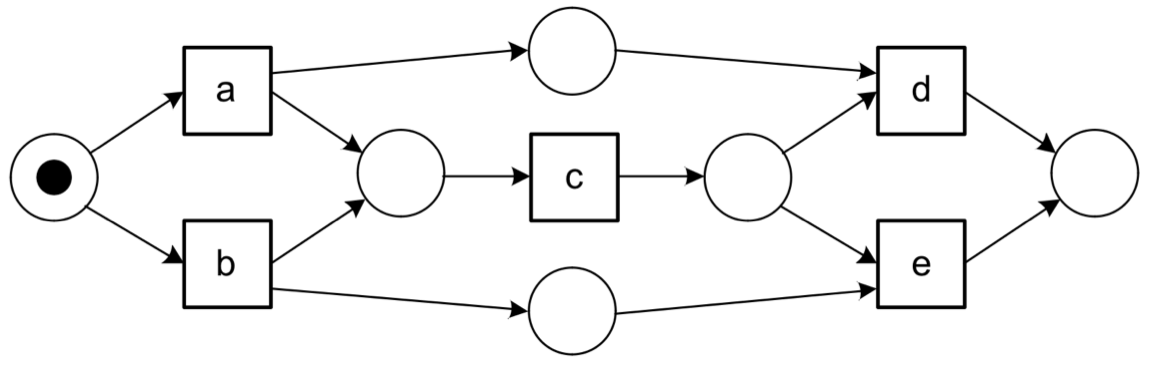
\includegraphics[width=0.4\textwidth]{../images/exercises/replay_based_3.png}
    \caption{Petri net for Exercise 3}
\end{figure}
\[L = [\langle a,c,d \rangle^{10}, \langle b,c,e \rangle^{10}], \langle a,c,e \rangle^{5}, \langle b,c,d \rangle^{5}, \langle d,c,a \rangle,\]
\[\langle a,b,d \rangle, \langle d \rangle] \]
Use replay-based conformance checking to compute the fitness of the event log with respect to the Petri net.
\end{exercise}
\paragraph{Solution:}

\begin{exercise}{4}
Given the following Petri net and event log:
\begin{figure}[H]
    \centering
    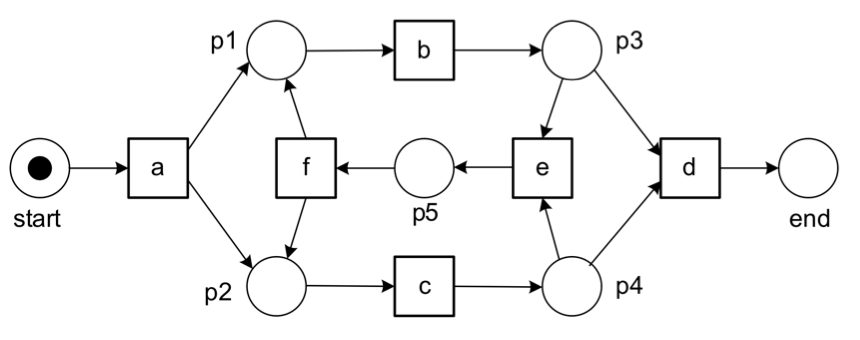
\includegraphics[width=0.4\textwidth]{../images/exercises/replay_based-4.png}
    \caption{Petri net for Exercise 4}
\end{figure}
\[L = [\langle a,b,e,f,c,d \rangle^{10}, \langle a,b,b,e,f,c,c,d \rangle^{10}]\]
Compute the fitness of the event log with respect to the Petri net using replay-based conformance checking.
\end{exercise}
\paragraph{Solution:}

\begin{exercise}{5}
Given the following Petri net and trace:
\begin{figure}[H]
    \centering
    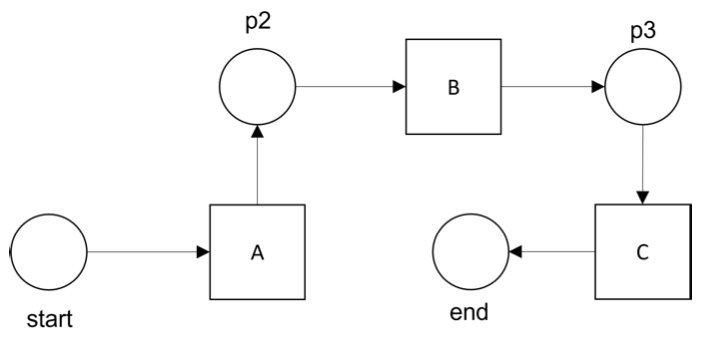
\includegraphics[width=0.4\textwidth]{../images/exercises/replay_based-5.png}
    \caption{Petri net for Exercise 5}
\end{figure}
Trace: $\langle a,b,b \rangle$
Compute the number of produced, consumed, missing, and remaining tokens.
\end{exercise}
\paragraph{Solution:}


\subsection{Alignment-based Conformance Checking}
\begin{exercise}{1}
Given the following Petri net and event log:
\begin{figure}[H]
    \centering
    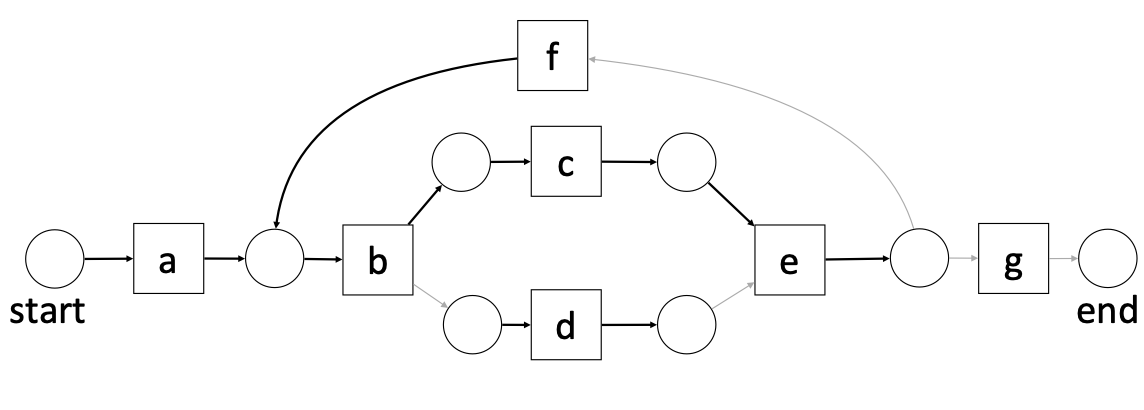
\includegraphics[width=0.4\textwidth]{../images/exercises/alignment-based_1.png}
    \caption{Petri net for Exercise 1}
\end{figure}
\[L = [\langle a,b,c,d,e,g \rangle^{10}, \langle a,b,c,e,f,e,g \rangle^{2}]\]
Use alignment-based conformance checking to compute the fitness of the event log with respect to the Petri net.
\end{exercise}
\paragraph{Solution:}
\begin{enumerate}
    \item First, we need to compute the fitness for each unique trace in the event log:
    \item For trace $\langle a,b,c,d,e,g \rangle$, suppose it matches perfectly with the process model:
    \begin{itemize}
        \item Optimal alignment cost = 0;
        \item To compute the worst-case alignment cost, we first need to make all log moves, resulting in a cost of 6 (one for each event in the trace);
        \item Then, we need to make all model moves in the shortest path from the initial to the final marking, which is 6.
    \begin{table}[H]
        \centering
        \begin{tabular}{|c|c|c|c|c|c|c|c|c|c|c|c|}
            \hline
            a & b & c & d & e & g & $\gg$ & $\gg$ & $\gg$ & $\gg$ & $\gg$ & $\gg$ \\
            \hline
            $\gg$ & $\gg$ & $\gg$ & $\gg$ & $\gg$ & $\gg$ & a & b & d & c & e & g \\ 
            \hline
        \end{tabular}
    \end{table}
        \item Worst-case alignment cost = 12;
        \item Fitness = $1 - \frac{0}{12} = 1$;
    \end{itemize}
    \item For trace $\langle a,b,c,e,f,e,g \rangle$:
    \begin{itemize}
        \item Optimal alignment cost = 3, 2 log moves (for $e$ and $f$) and 1 model move (for $d$);
        \begin{table}[H]
            \centering
            \begin{tabular}{|c|c|c|c|c|c|c|c|}
                \hline
                a & b & c & $\gg$ & e & f & e & g \\
                \hline
                a & b & c & d & $\gg$ & $\gg$ & e & g \\
                \hline
            \end{tabular}
        \end{table}
        \item Worst-case alignment cost = 13, 7 log moves and 6 model moves;
    \end{itemize}
    \item Finally, we can compute the fitness of the event log as the weighted average of the fitness of each trace:
    \[fitness(L, N) = \frac{10 \times 1 + 2 \times 0.75}{10 + 2} = \frac{11.5}{12} \approx 0.96\]
\end{enumerate}
